\begin{frame}
\frametitle{About This Work...}

\emph{Scalable Continuous Range Monitoring of Moving Objects in Symbolic Indoor Space}.~\cite{DBLP:conf/cikm/YangLJ09} \\
B.~Yang, H.~Lu, and C.~S. Jensen.\\~\\

\begin{itemize}
  \item Published in \emph{CIKM' 2009}.
  \item Application: continuously monitor indoor moving objects for space use analysis or security purposes.
  \item An incremental, query-aware continuous range query processing technique for objects moving in indoor space.
  \item Use maxmum-speed constraint on object movement to refine the uncertain results.
\end{itemize}

\end{frame}
%------------------------------------------------

\begin{frame}
\frametitle{Motivation}

\begin{itemize}
  \item People spend much time in indoor spaces.

  \item Indoor spaces are becoming increasingly larger and complex.
    \begin{itemize}
      \item E.g., London Underground, 268 stations, 408 kilometers of network, +4 million daily passegers.
    \end{itemize}

  \item Indoor monitoring of people can help support.
    \begin{itemize}
      \item space use analysis
      \item security purposes
    \end{itemize}
\end{itemize}

\end{frame}

%------------------------------------------------

\begin{frame}
\frametitle{Preliminaries: Indoors vs. Outdoors}

\begin{itemize}
  \item Modeling of indoor spaces do not assume
    \begin{itemize}
      \item Euclidean space. (since obstacles render movement more constrained)
      \item Spatial network. (since indoor movement is less constrained than movements in polylines)
    \end{itemize}

  \item Instead indoor spaces are characterized by entities.
    \begin{itemize}
      \item Doors, rooms, hallways, staircase, etc.
    \end{itemize}

  \item \textbf{Symbolic models} are more suitable.

  \item \emph{GPS} and \emph{cellular tracking} do not work indoors.

  \item Sensing devices are used to detect objects within their activation range, e.g., RFID readers or Bluetooth hotspots.
\end{itemize}

\end{frame}

%------------------------------------------------

\begin{frame}
\frametitle{Positioning Devices Deployment Graph}

\begin{columns}[c]

  \column{.57\textwidth}
  \begin{itemize}
    \footnotesize{
    %\item More advanced compared to \emph{RFID Deployment Graph}.
    \item Two types of positioning devices
      \begin{itemize}
        \scriptsize{
        \item Partitioning Device -- \emph{undirected} (\textbf{UP}), e.g., $\mathnormal{d_{21}}$ -- \emph{directed} (\textbf{DP}), e.g., $\mathnormal{d_{11}}$ and $\mathnormal{d_{11'}}$
        \item Presence Device -- (\textbf{PR})
        }
      \end{itemize}
    \item Note an indoor space is partitioned into \emph{activation ranges} and \emph{cells}
    }
  \end{itemize}
  \begin{block}{Deployment Graph}
    \textrm{
    \begin{itemize}
      \scriptsize{
      \item $\mathnormal{G = \{C, E, \Sigma_{devices}, l_E\}}$
      \item $\mathnormal{C}$: the set of cells
      \item $\mathnormal{E}$: the set of edges, $\mathnormal{\{ c_i, c_j \}}$ where $\mathnormal{c_i, c_j \in C}$
      \item $\mathnormal{\Sigma_{devices}}$: a mapping from $\mathnormal{deviceID}$ to activation range and type
      \item $\mathnormal{l_E}$ maps an edge to a set of positioning devices, i.e., $\mathnormal{E \rightarrow 2^{\Sigma_{devices}}}$
      }
    \end{itemize}
    }
  \end{block}

  \column{.43\textwidth}
    \vspace{-30pt}
    \begin{figure}[tb]
      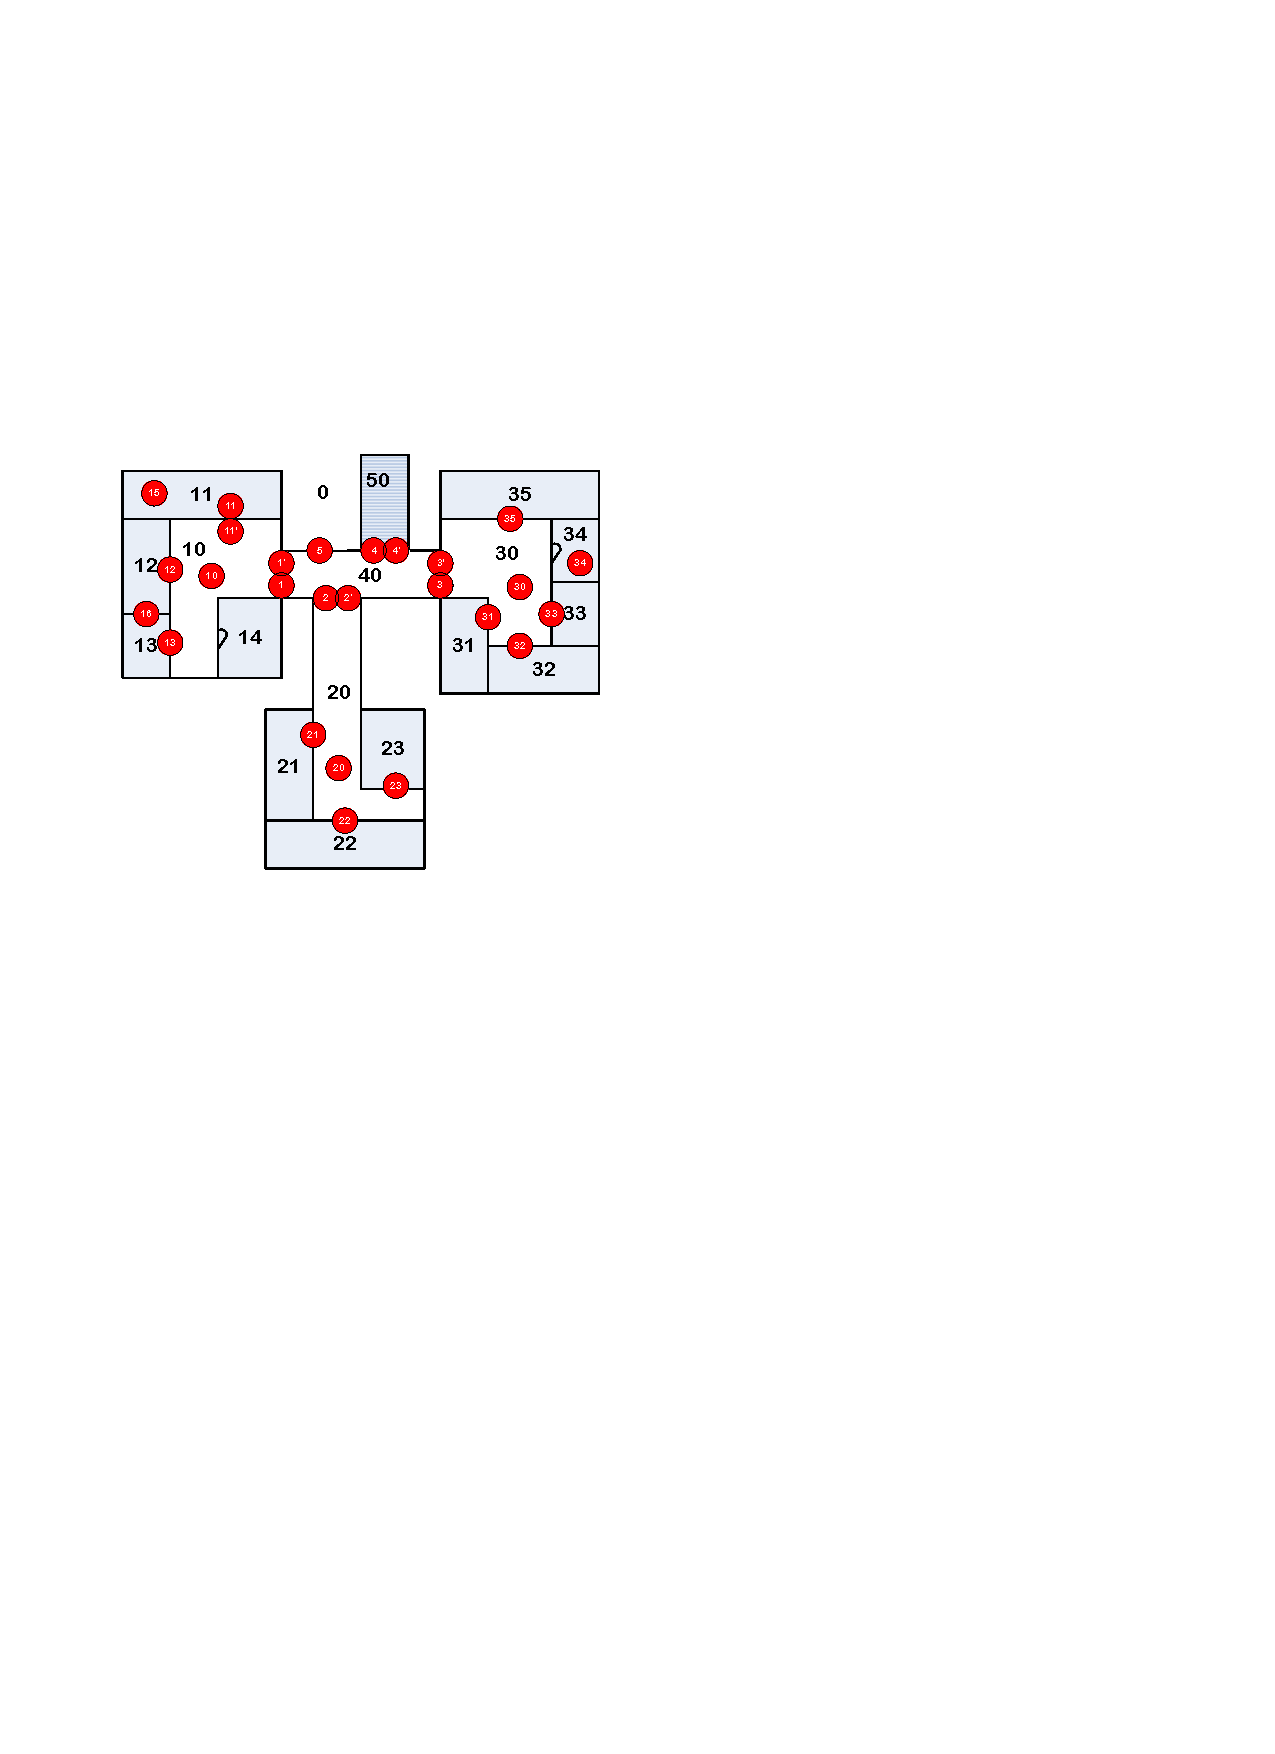
\includegraphics[width=\columnwidth]{figures/2-2-1.pdf}
    \end{figure}
    \vspace{-20pt}
    \pause
    \begin{figure}[tb]
      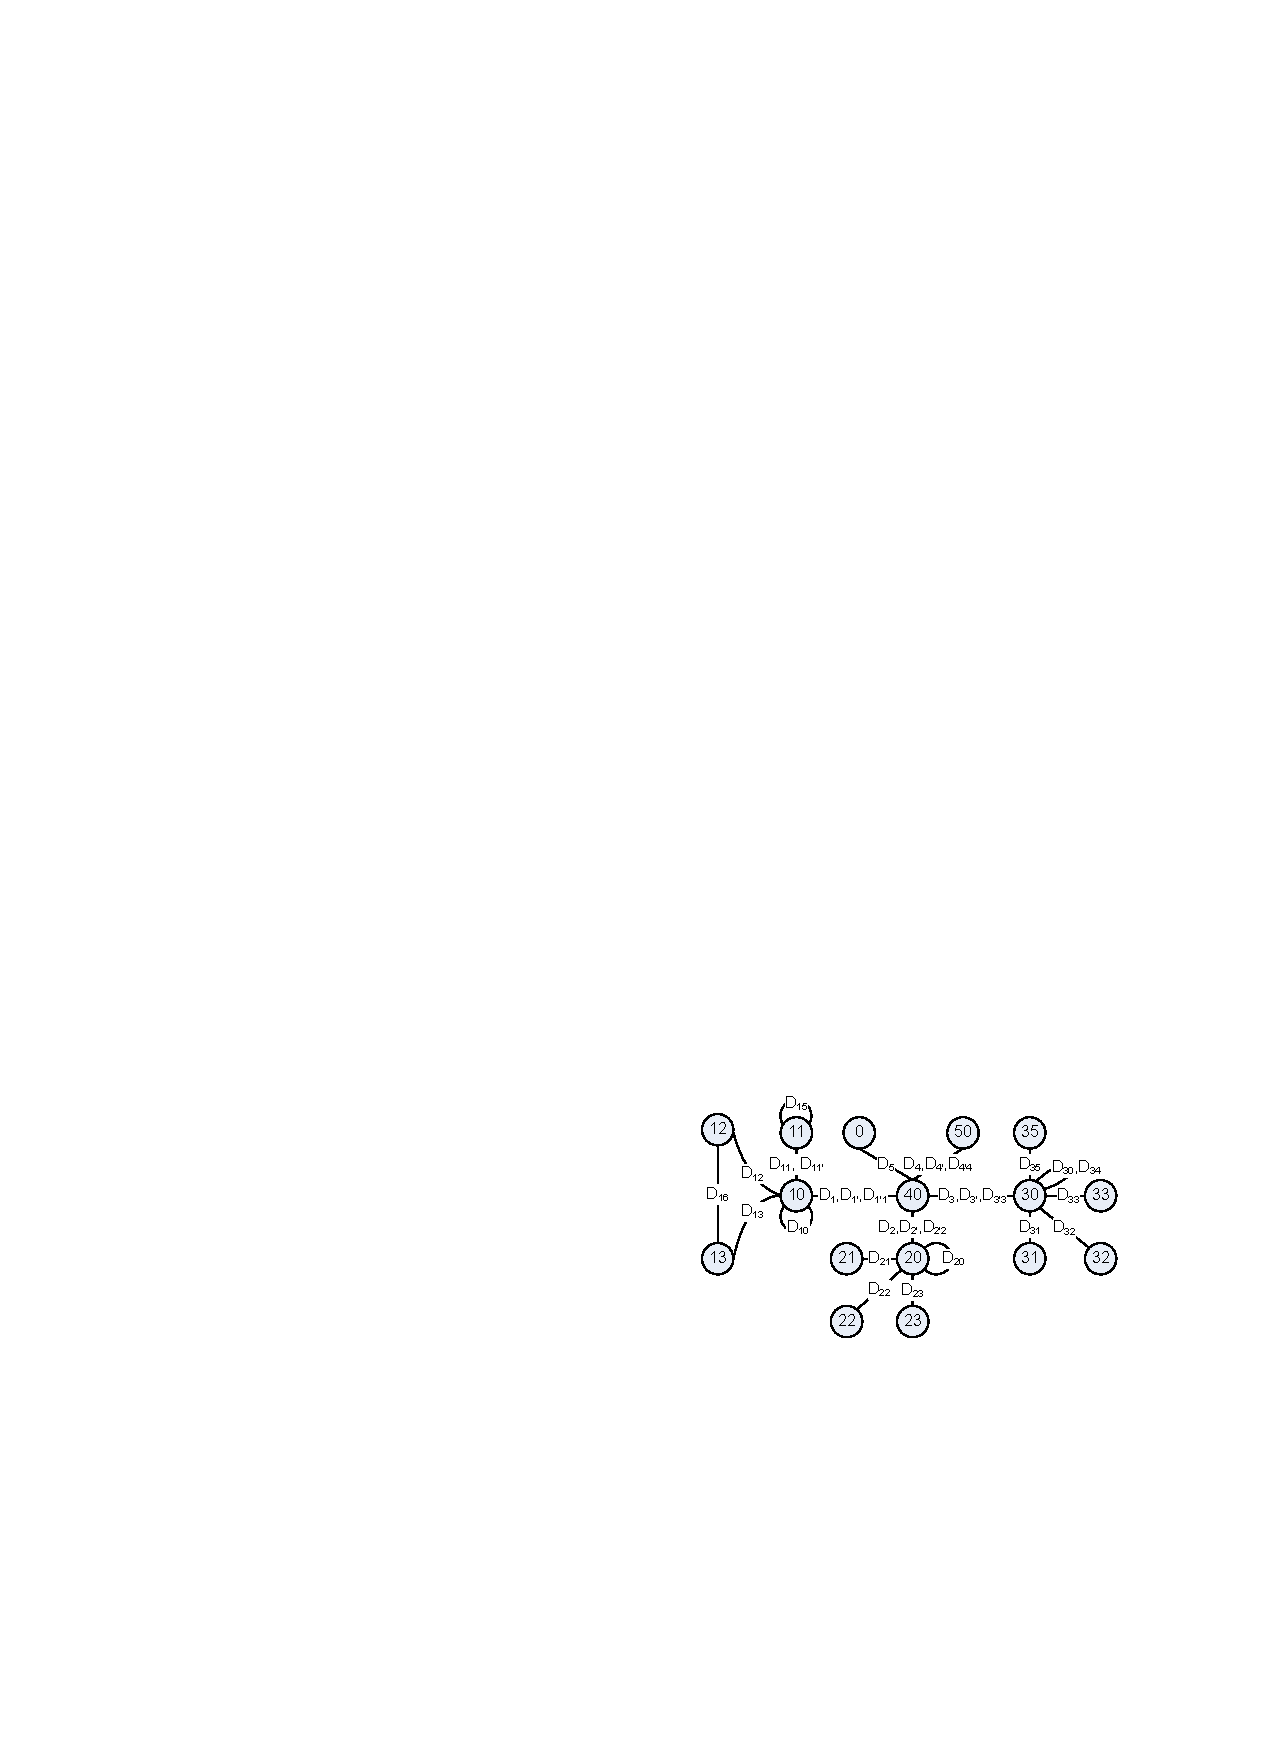
\includegraphics[width=\columnwidth]{figures/2-2-2.pdf}
    \end{figure}

\end{columns}

\end{frame}
